\clearpage
\section{BPSK Transmission System}

\begin{tcolorbox}	
\begin{tabular}{p{2.75cm} p{0.2cm} p{10.5cm}} 	
\textbf{Student Name}  &:& Daniel Pereira\\
\textbf{Starting Date} &:& September 1, 2017\\
\textbf{Goal}          &:& Binary Phase Shift Keying with additive white Gaussian noise.
\end{tabular}
\end{tcolorbox}

Binary Phase Shift Keying (BPSK) is the simplest form of Phase Shift Keying (PSK), in which binary information is encoded into a two state constellation with the states being separated by a phase shift of $\pi$.
\par
White Noise (WN) is a random signal with equal intensity at all frequency, having a constant power spectral density. WN is said to be Gaussian (WGN) if it's samples follow a normal distribution with zero mean and a certain variance $\sigma^2$. For WGN we know it's spectral density to be equal to it's variance, therefore we can choose $\sigma^2$ in accordance with the desired spectral density.
\par
The purpose of this system is to simulate BPSK transmission in back-to-back configuration with additive WGN at the receiver.

\subsection{BER of BPSK with additive WGN}

The output of the system with added gaussian noise is expected to follow a normal distribution, whose first probabilistic moment can be readily obtained by knowledge of the optical power of the two inputs:
\begin{equation}\label{eq:mu1}
\mu=2\sqrt{P_LP_S}Amp\cos(\Delta\theta),
\end{equation}
where $P_L$ and $P_S$ are the optical powers, in watts, of the local oscillator and signal, respectively, $Amp$ is the amplification factor chosen in the homodyne receiver and $\Delta\theta$ is the phase difference between the local oscillator and the signal, for BPSK this can be assumed to take the values $\pi$ and 0, in which case~\eqref{eq:mu1} can be reduced to:
\begin{equation}
\mu=\pm2\sqrt{P_LP_S}Amp.
\end{equation}
The second moment is directly chosen by inputting the spectral density of the noise $\sigma^2$, and thus is known \textit{a priori}.
\par
Both probabilist moments being known, the probability distribution of measurement results is given by a simple normal distribution:
\begin{equation}
f(x)=\frac{1}{\sqrt{2\pi}\sigma}e^{-\frac{(x-\mu)^2}{2\sigma^2}}.
\end{equation}
The BER is calculated in the following manner:
\begin{equation}
BER=\frac{1}{2}\int_0^{+\infty}f(x|\Delta\theta=\pi)\text{d}x+\frac{1}{2}\int^0_{-\infty}f(x|\Delta\theta=0)\text{d}x,
\end{equation}
given the symmetry of the system, this can be simplified to:
\begin{equation}\label{eq:BERtheoretical}
BER=\int_0^{+\infty}f(x|\Delta\theta=\pi)\text{d}x=\frac{1}{2}\text{erfc}\left(\frac{-\mu}{\sqrt{2}\sigma}\right)
\end{equation}

\subsection{Simulation}

A simplified diagram of the system being simulated is presented in the Figure~\ref{fig:homodynesystem}. A random binary string is generated and encoded in an optical signal using BPSK modulation. The decoding of the optical signal is accomplished by an homodyne receiver, which combines the signal with a local oscillator. The received binary signal is compared with the transmitted binary signal in order to estimate the Bit Error Rate (BER). The simulation is repeated for multiple signal power levels, each corresponding BER is recorded and plotted against the expectation value.

\begin{figure}[h]
\centering
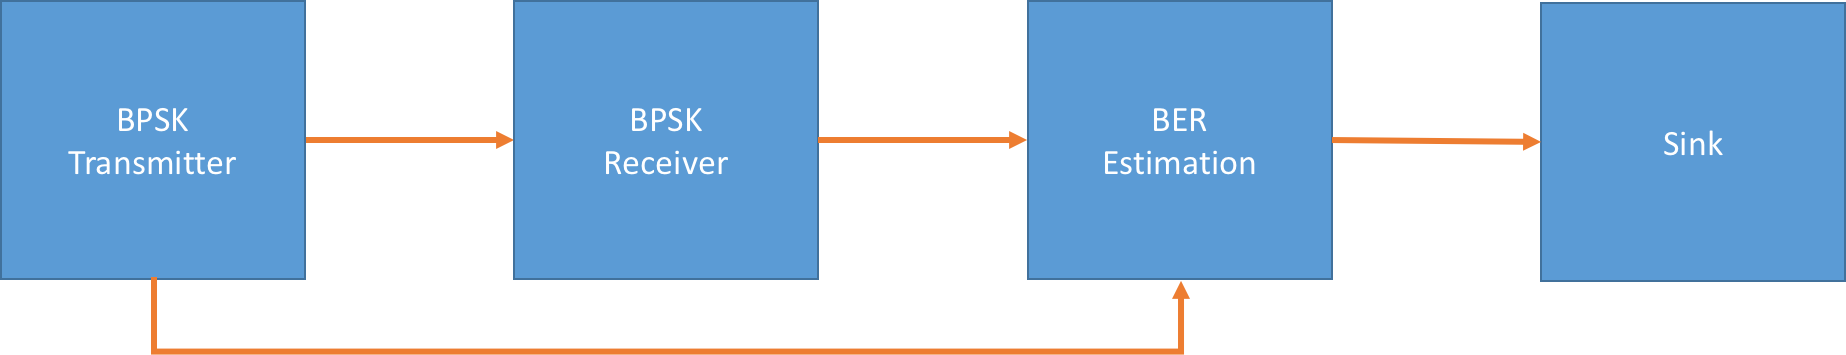
\includegraphics[width=\linewidth]{bpskdiagram.png}
\caption{Overview of the BPSK system being simulated.}
\label{fig:homodynesystem}
\end{figure}

\begin{table}[H]
\centering
\begin{tabular}{c|c}
System Blocks    & netxpto Blocks   \\ \hline
BPSK Transmitter & MQamTransmitter  \\
BPSK Receiver    & HomodyneReceiver \\
BER Estimator    & BitErrorRate
\end{tabular}
\end{table}

\subsection*{Required files}\label{Required files}

Header Files

\begin{table}[H]
\centering
\begin{tabulary}{1.0\textwidth}{|L|L|}
\hline
\textbf{File}              & \textbf{Description} 				                  \\ \hline
netxpto.h                  & Generic purpose simulator definitions.	              \\ \hline
m\_qam\_transmitter.h      & Generates the signal with coded constellation.       \\ \hline
local\_oscillator.h        & Generates a continuous optical signal with set power and phase. \\ \hline
balanced\_beam\_splitter.h & Mixes the two optical signals set at it's input. \\ \hline
homodyne\_reciever.h       & Performs coherent detection on the input signal.     \\ \hline
sampler.h                  & Samples the input signal at a user defined frequency. \\ \hline
bit\_decider.h             & Decodes the input signal into a binary string.       \\ \hline
bit\_error\_rate.h         & Calculates the bit error rate of the decoded string. \\ \hline
sink.h                     & Closes any unused signals.                           \\ \hline
\end{tabulary}
\end{table}		
%
Source Files
\begin{table}[H]
\centering
\begin{tabulary}{1.0\textwidth}{|L|L|}
\hline
\textbf{File}           & \textbf{Description} 					             \\ \hline
netxpto.cpp             & Generic purpose simulator implementations.           \\ \hline
m\_qam\_transmitter.cpp &  Generates the signal with coded constellation.      \\ \hline
local\_oscillator.cpp   & Generates a continuous optical signal with set power and phase \\ \hline
balanced\_beam\_splitter.h & Mixes the two optical signals set at it's input. \\ \hline
homodyne\_reciever.cpp  & Performs coherent detection on the input signal.     \\ \hline
sampler.cpp             & Samples the input signal at a user defined frequency. \\ \hline
bit\_decider.cpp        & Decodes the input signal into a binary string.       \\ \hline
bit\_error\_rate.cpp    & Calculates the bit error rate of the decoded string. \\ \hline
sink.cpp                & Closes any unused signals.                           \\ \hline
\end{tabulary}
\end{table}		

\subsection*{System Input Parameters}

This system takes into account the following input parameters:

\begin{table}[H]
\centering
\begin{tabulary}{1.0\textwidth}{|C|C|}
\hline
\textbf{System Parameters} & \textbf{Description} 																 \\ \hline
numberOfBitsGenerated      & Gives the number of bits to be simulated		          										 \\ \hline
bitPeriod                  & Sets the time between adjacent bits                                                           \\ \hline
samplesPerSymbol           & Establishes the number of samples each bit in the string is given 	         \\ \hline
pLength                    & PRBS pattern length					                      									 \\ \hline
iqAmplitudesValues         & Sets the state constellation																	 \\ \hline
outOpticalPower\_dBm       & Sets the optical power, in units of dBm, at the transmitter output							 \\ \hline
loOutOpticalPower\_dBm     & Sets the optical power, in units of dBm, of the local oscillator used in the homodyne detector \\ \hline
localOscillatorPhase       & Sets the initial phase of the local oscillator used in the homodyne detector					 \\ \hline
transferMatrix             & Sets the transfer matrix of the beam splitter used in the homodyne detector					 \\ \hline
responsivity               & Sets the responsivity of the photodiodes used in the homodyne detector						 \\ \hline
amplification              & Sets the amplification of the trans-impedance amplifier used in the homodyne detector			 \\ \hline
noiseSpectralDensity       & Sets the spectral density of the gaussian thermal noise added in the homodyne detector		 \\ \hline
confidence                 & Sets the confidence interval for the calculated QBER                                           \\ \hline
midReportSize              & Sets the number of bits between generated QBER mid-reports                                     \\ \hline
\end{tabulary}
\end{table}		

\subsection*{Inputs}

This system takes no inputs.

\subsection*{Outputs}

This system outputs the following objects:
\begin{itemize}
\item Signals:
\begin{itemize}
\item Initial Binary String; (S$_0$)
\item Optical Signal with coded Binary String; (S$_{1}$)
\item Local Oscillator Optical Signal; (S$_{2}$)
\item Beam Splitter Outputs; (S$_{3}$, S$_{4}$)
\item Homodyne Detector Electrical Output; (S$_{5}$)
\item Decoded Binary String; (S$_{6}$)
\item BER result String; (S$_{7}$)
\end{itemize}
\item Other:
\begin{itemize}
\item Bit Error Rate report in the form of a .txt file. (BER.txt)
\end{itemize}
\end{itemize}

\subsection*{Simulation Results}

The following results show the dependence of the error rate with the signal power assuming a constant Local Oscillator power of $0~dBm$, the signal power was evaluated at levels between -70~and~-25~dBm, in steps of 5~dBm between each. The simulation results are presented in orange with the computed lower and upper bounds, while the expected value, obtained from~\eqref{eq:BERtheoretical}, is presented as a full blue line. A close agreement is observed between the simulation results and the expected value. The noise spectral density was set at $\sqrt{2}*0.0005$~V$^2$. 
\begin{figure}[H]
\centering
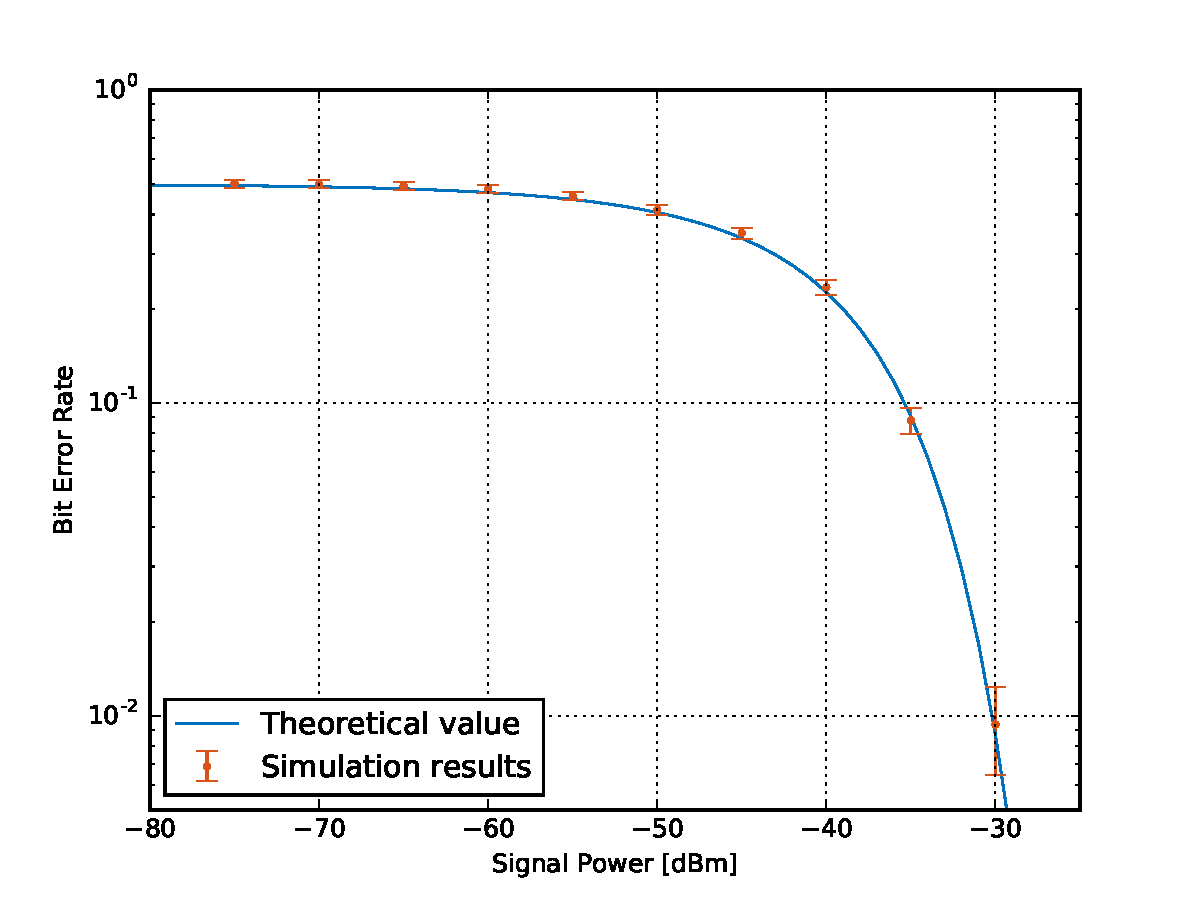
\includegraphics[width=\linewidth]{BER_Evolution.pdf}
\caption{Bit Error Rate in function of the signal power in dBm.}
\label{fig:berevolution}
\end{figure}

\begin{figure}[H]
\centering
\begin{subfigure}{.3\linewidth}
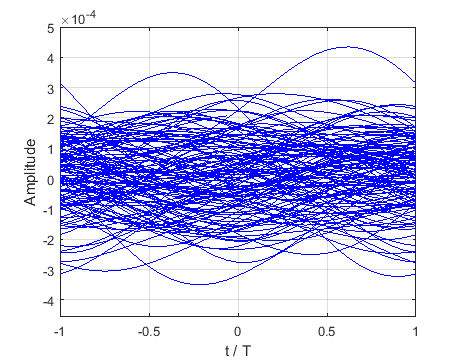
\includegraphics[width=\linewidth]{eyeclosed.png}
\caption{Power=-180dBm}
\end{subfigure}
\begin{subfigure}{.3\linewidth}
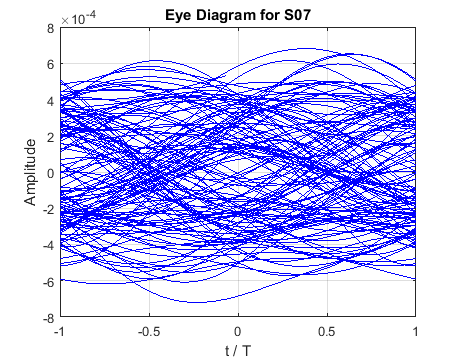
\includegraphics[width=\linewidth]{eyepartial.png}
\caption{Power=-130dBm}
\end{subfigure}
\begin{subfigure}{.3\linewidth}
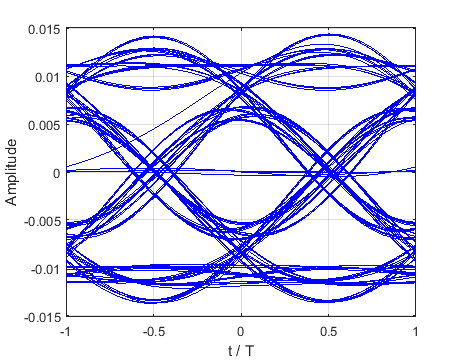
\includegraphics[width=\linewidth]{eyeopen.png}
\caption{Power=-100dBm}
\end{subfigure}
\caption{Eye diagrams at different signal powers.}
\end{figure}


%\section{Simulation Results}
%
%We consider the following scenarios:
%\begin{itemize}
%\item \ref{subsec:scenario1} Basic BPSK back to back with  thermal noise.
%\end{itemize}
%
%\subsection{BPSK with thermal noise}\label{subsec:scenario1}
%
%The following results were obtained from the simulation using the following input parameters:
%\begin{table}[H]
%\centering
%\begin{tabular}{rl}
%numberOfBits=           & 1000                                                     \\
%samplesPerSymbol=       & 16                                                       \\
%pLength=                & 5                                                        \\
%iqAmplitudesValues=     & \{ \{ 1, 0 \}, \{ -1, 0 \} \}                            \\
%outOpticalPower\_dBm=   & -20                                                      \\
%loOutOpticalPower\_dBm= & -10                                                      \\
%localOscillatorPhase=   & 0                                                        \\
%transferMatrix=         & \{ \{ 1/sqrt(2), 1/sqrt(2), 1/sqrt(2), -1/sqrt(2) \} \}  \\
%responsivity=           & 1                                                        \\
%amplification=          & 1e6                                                      \\
%noiseAmplitude=         & 15.397586549153788                                       \\
%delay=                  & 9                                                        \\
%\end{tabular}
%\end{table}
%
%The system took the binary string presented in Figure~\ref{fig:sentkey} and encoded it into the optical signal in Figure~\ref{fig:sentsig}. Notice the BPSK constelation of the signal, presented in Figure~\ref{fig:constellation}.
%\begin{figure}[H]
%\centering
%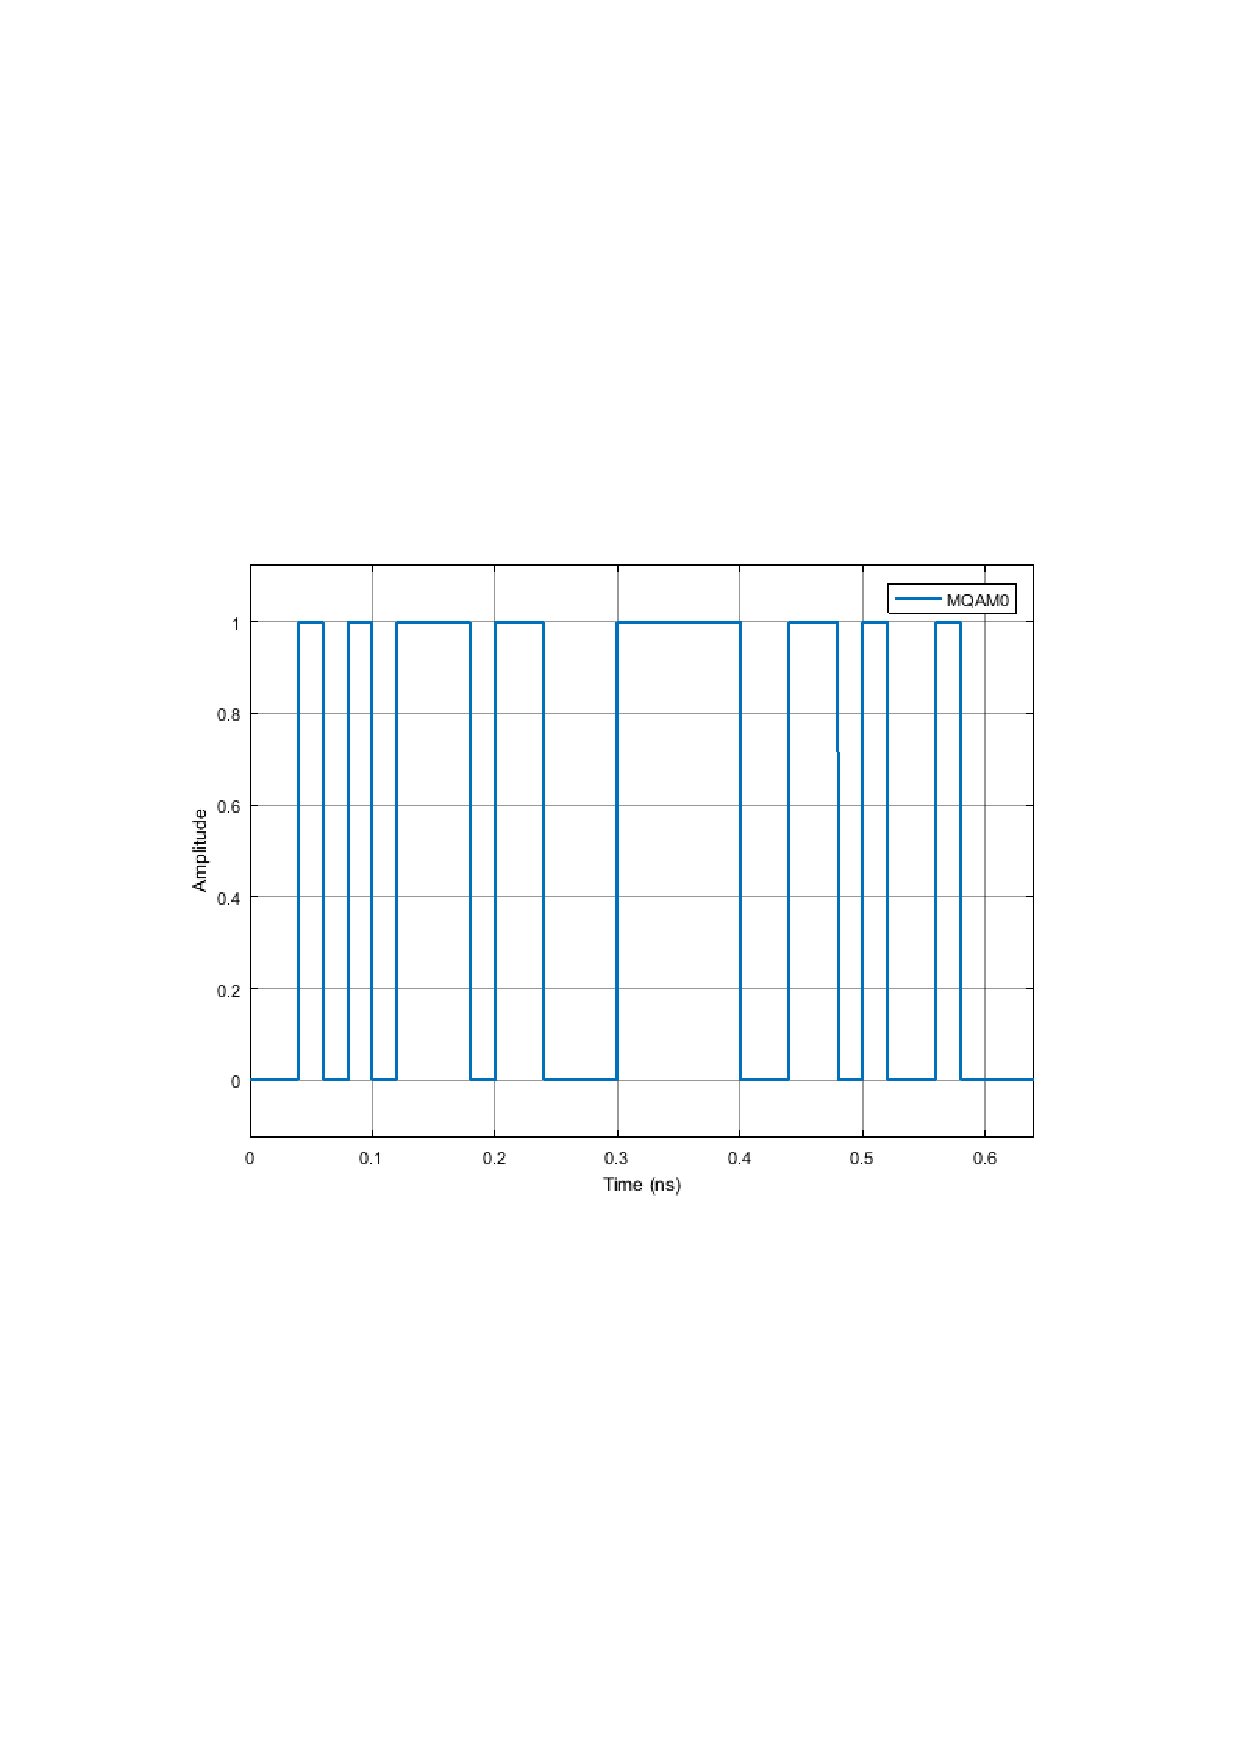
\includegraphics[width=\linewidth, trim= 0mm 95mm 0mm 95mm, clip]{binarystring.pdf}
%\caption{Sent binary key.}
%\label{fig:sentkey}
%\end{figure}
%
%\begin{figure}[H]
%\centering
%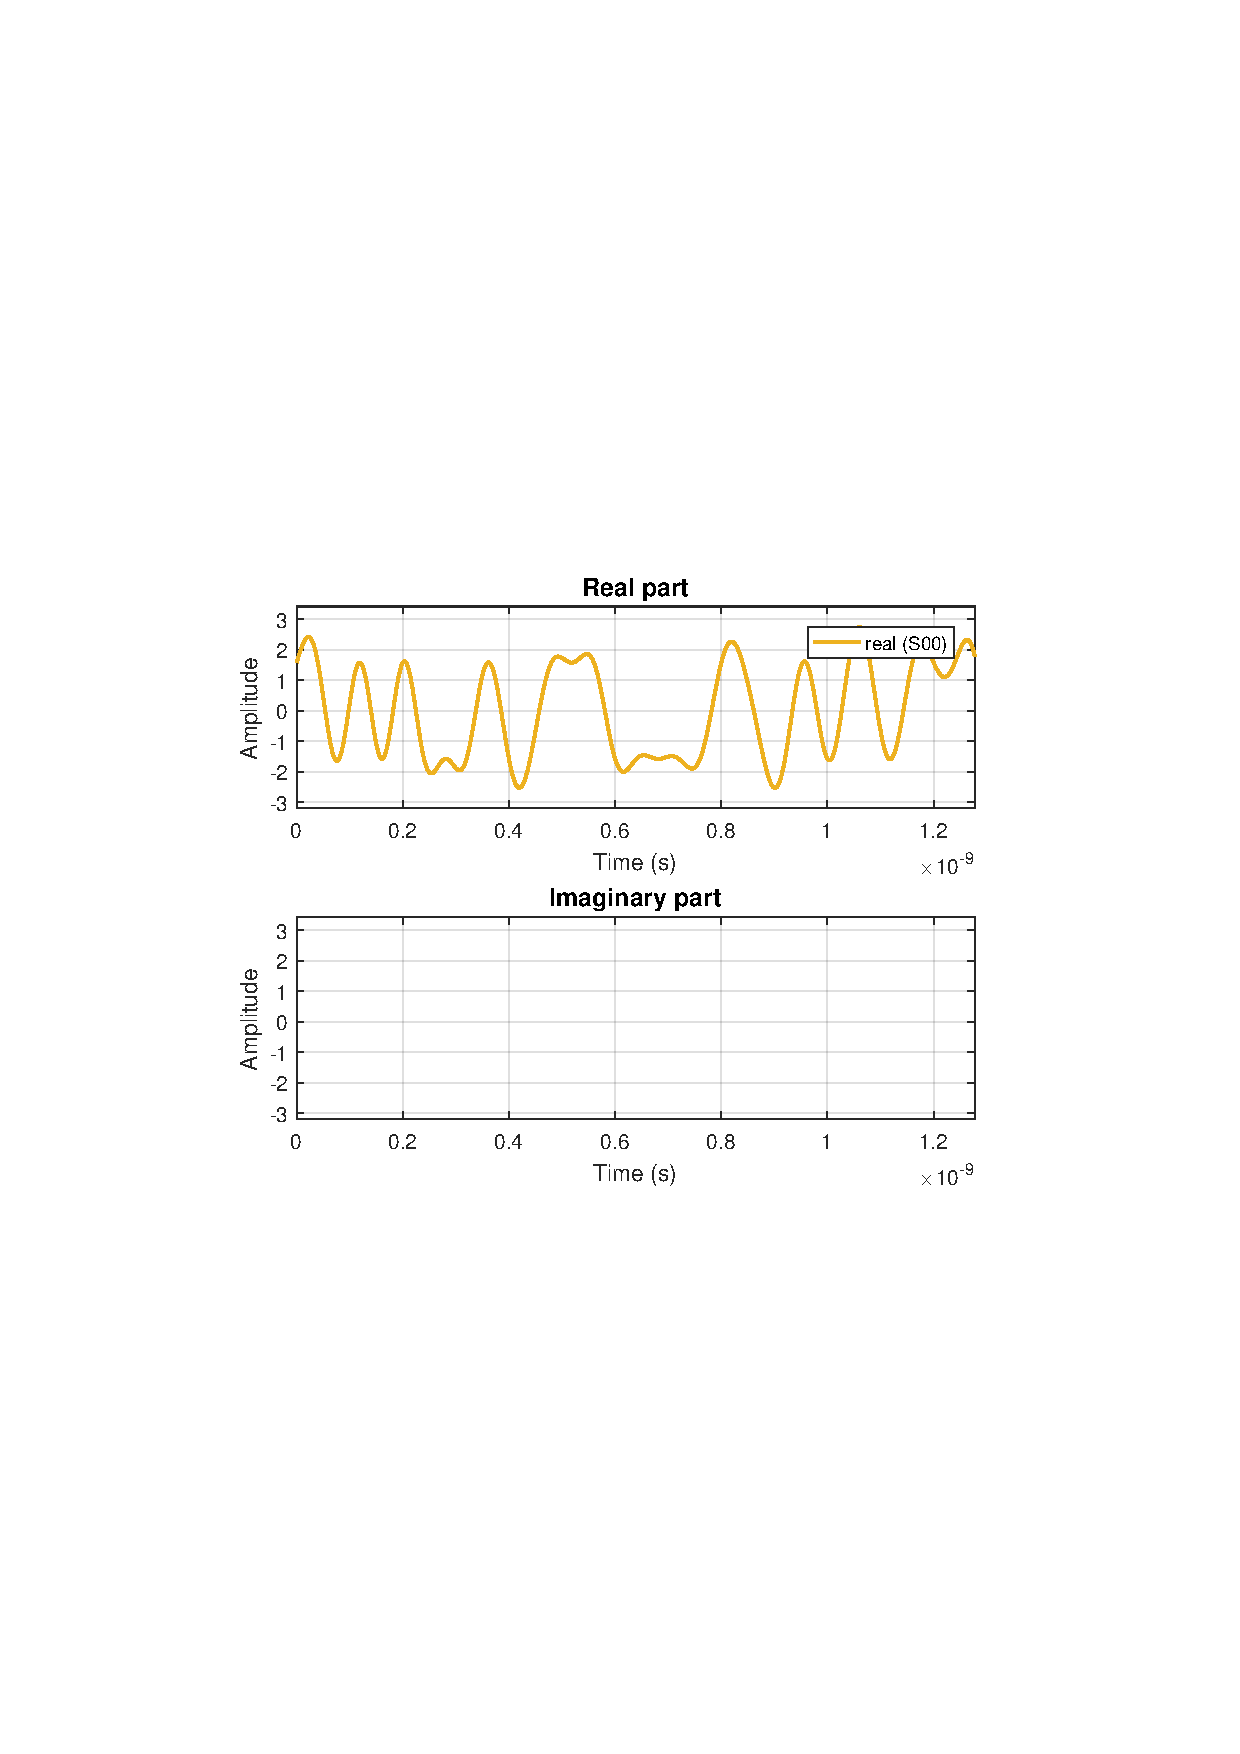
\includegraphics[width=\linewidth, trim= 0mm 95mm 0mm 95mm, clip]{sentsignal.pdf}
%\caption{Sent signal.}
%\label{fig:sentsig}
%\end{figure}
%
%\begin{figure}[H]
%\centering
%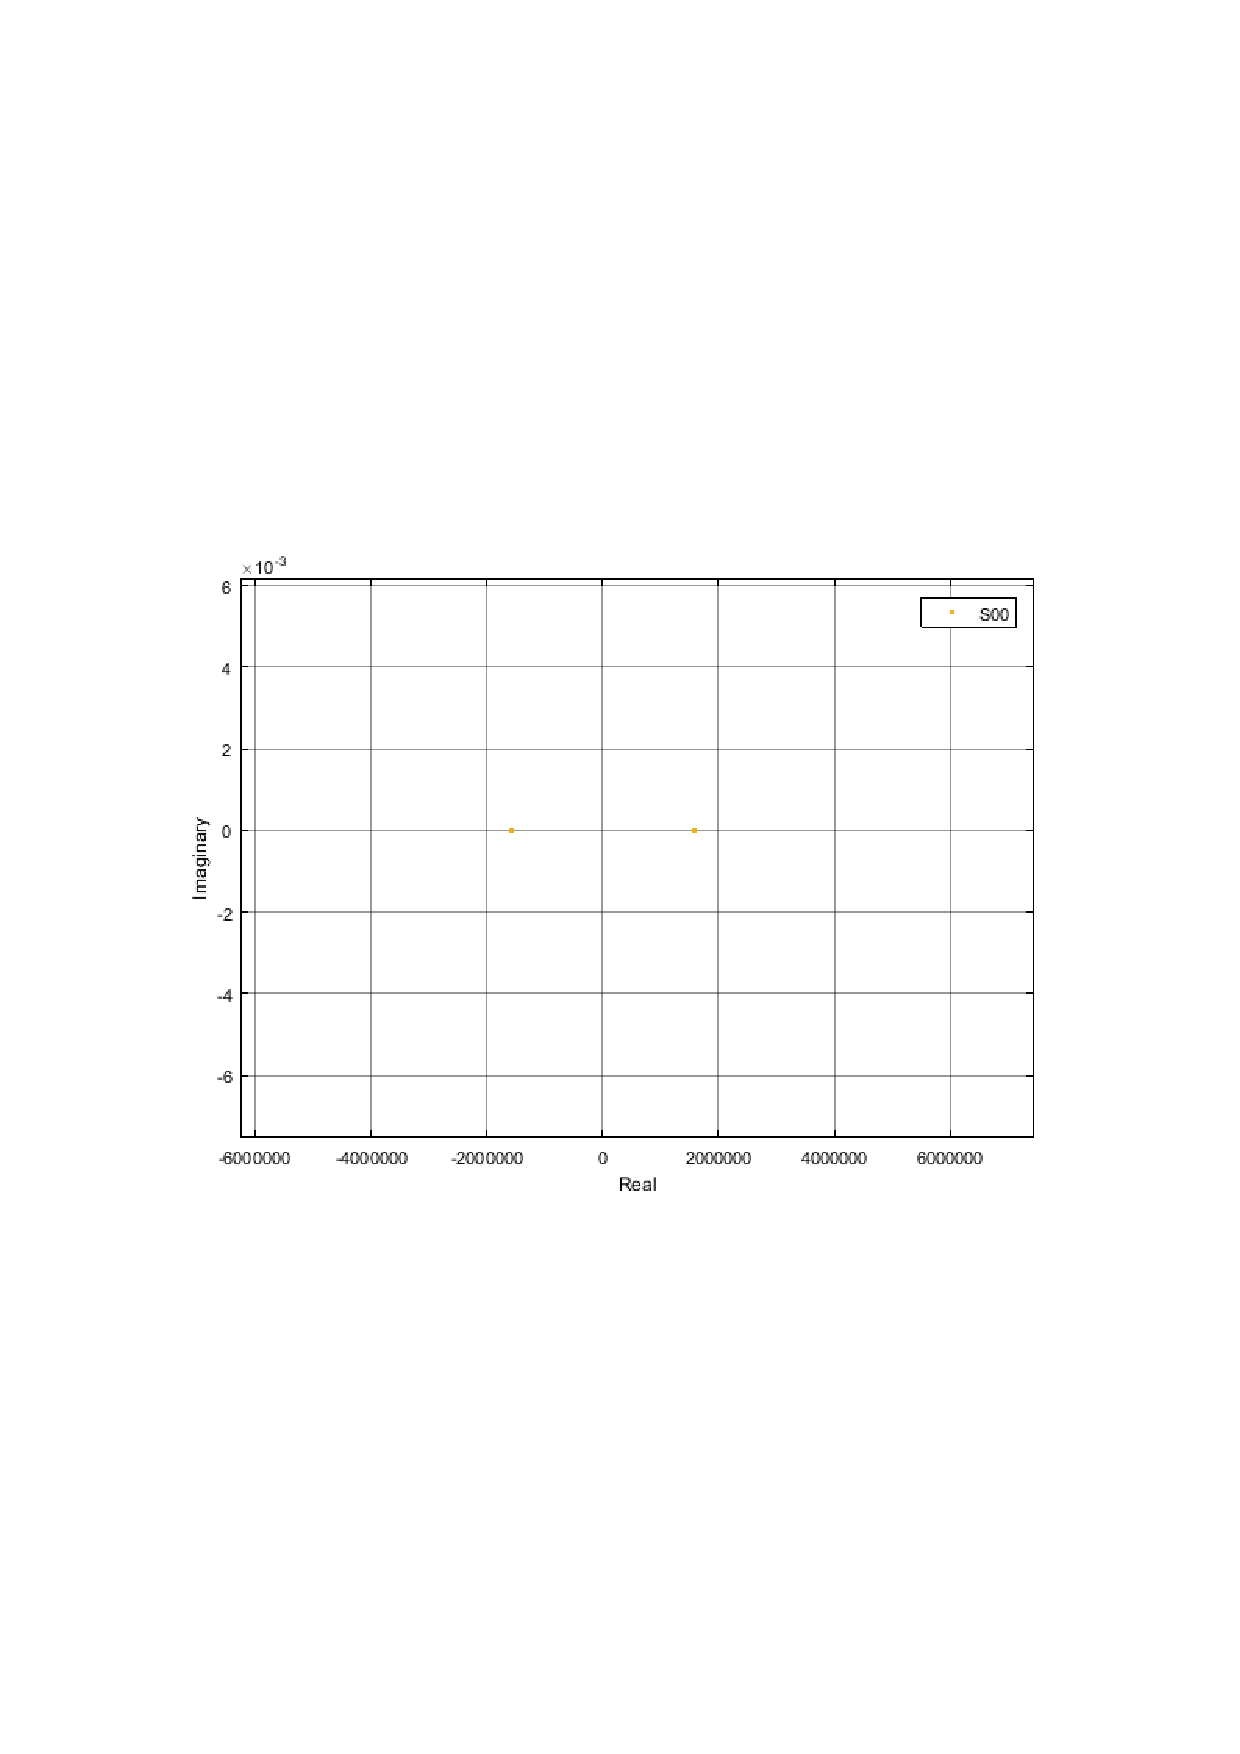
\includegraphics[width=\linewidth, trim= 0mm 95mm 0mm 95mm, clip]{constellation.pdf}
%\caption{Constellation of the sent signal.}
%\label{fig:constellation}
%\end{figure}
%
%Homodyne detection is then performed, using to that effect the local oscillator signal presented in Figure~\ref{fig:local}. Figures~\ref{fig:subtract}~and~\ref{fig:noisy} show the addition of noise to the signal.

%\begin{figure}[H]
%\centering
%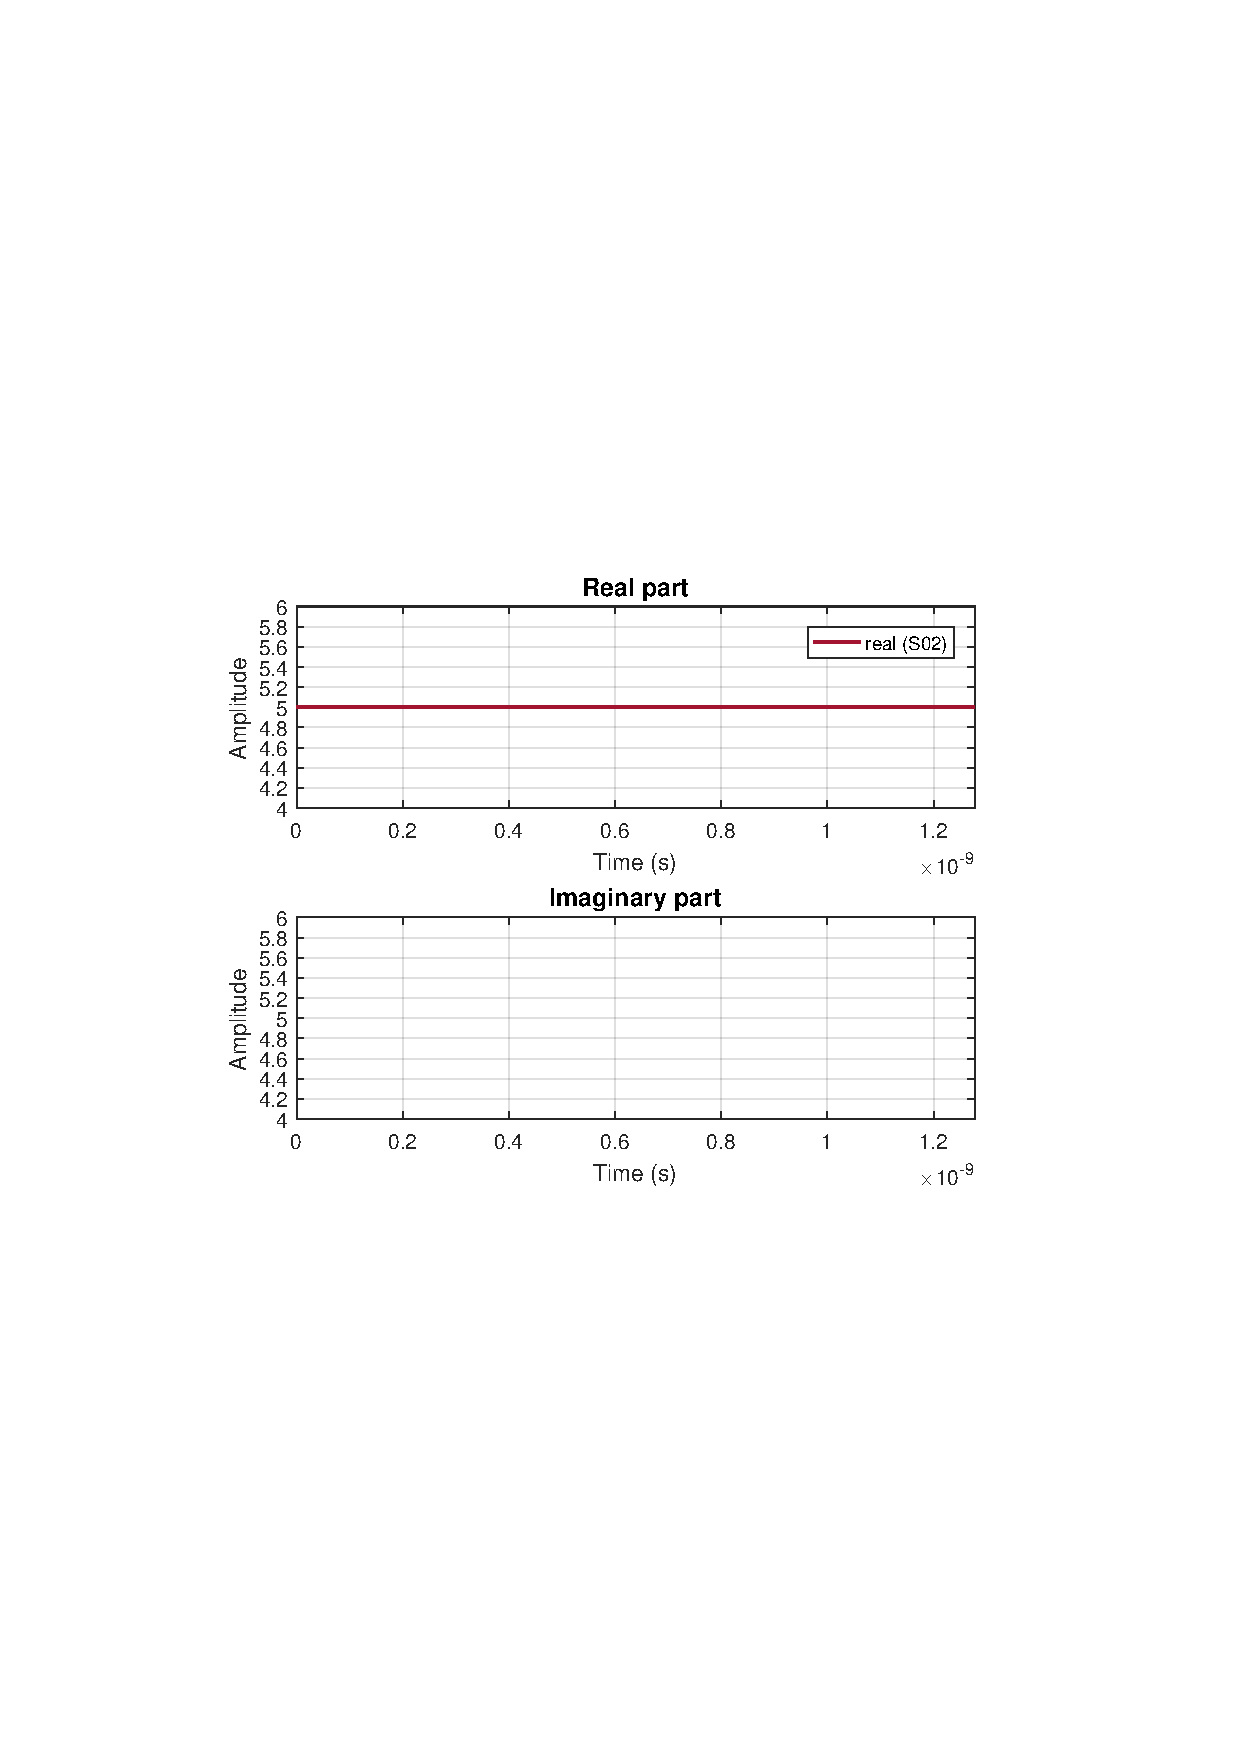
\includegraphics[width=\linewidth, trim= 0mm 95mm 0mm 95mm, clip]{localosc.pdf}
%\caption{Homodyne receiver internal signal: local oscillator used for Homodyne detection.}
%\label{fig:local}
%\end{figure}
%
%\begin{figure}[H]
%\centering
%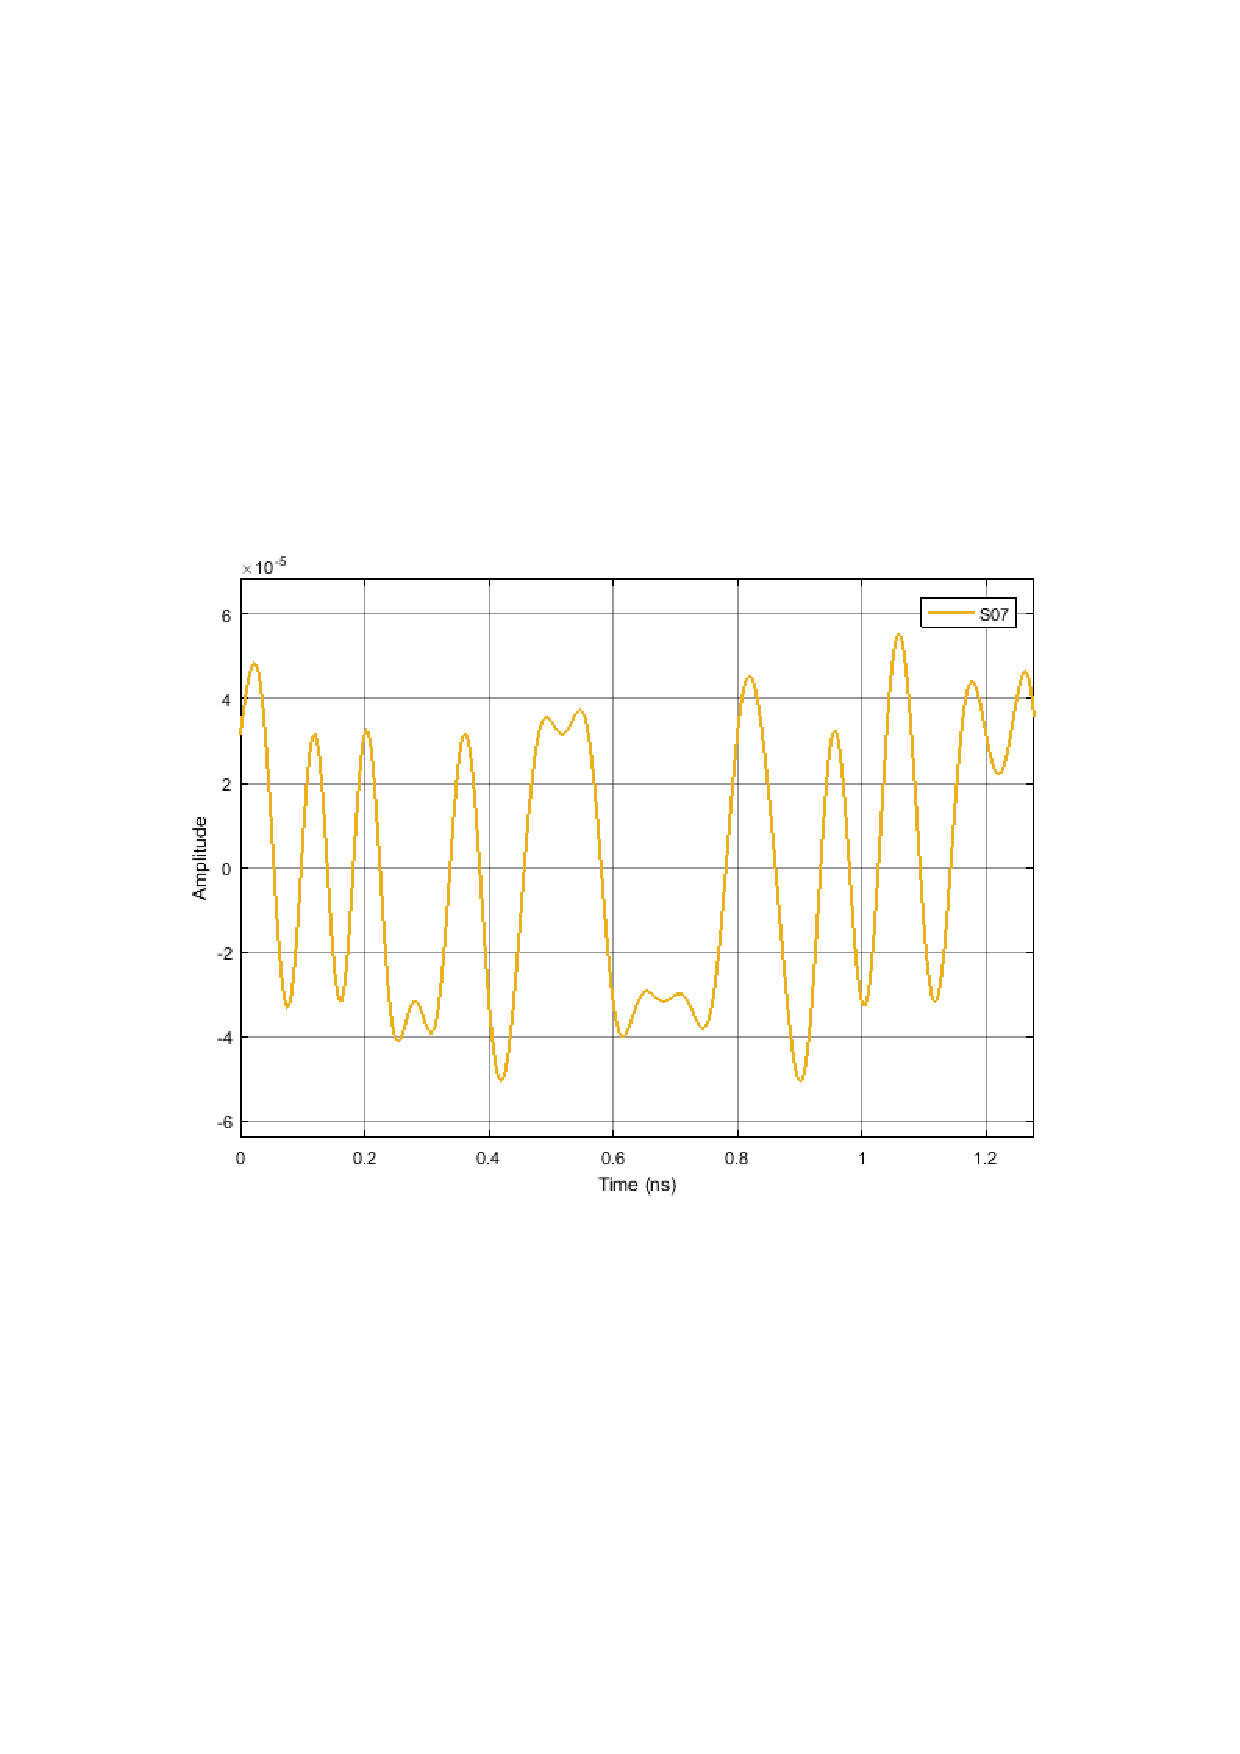
\includegraphics[width=\linewidth, trim= 0mm 95mm 0mm 95mm, clip]{subtract.pdf}
%\caption{Homodyne receiver internal signal: subtraction of the signals outputted by the photodiodes.}
%\label{fig:subtract}
%\end{figure}

%\begin{figure}[H]
%\centering
%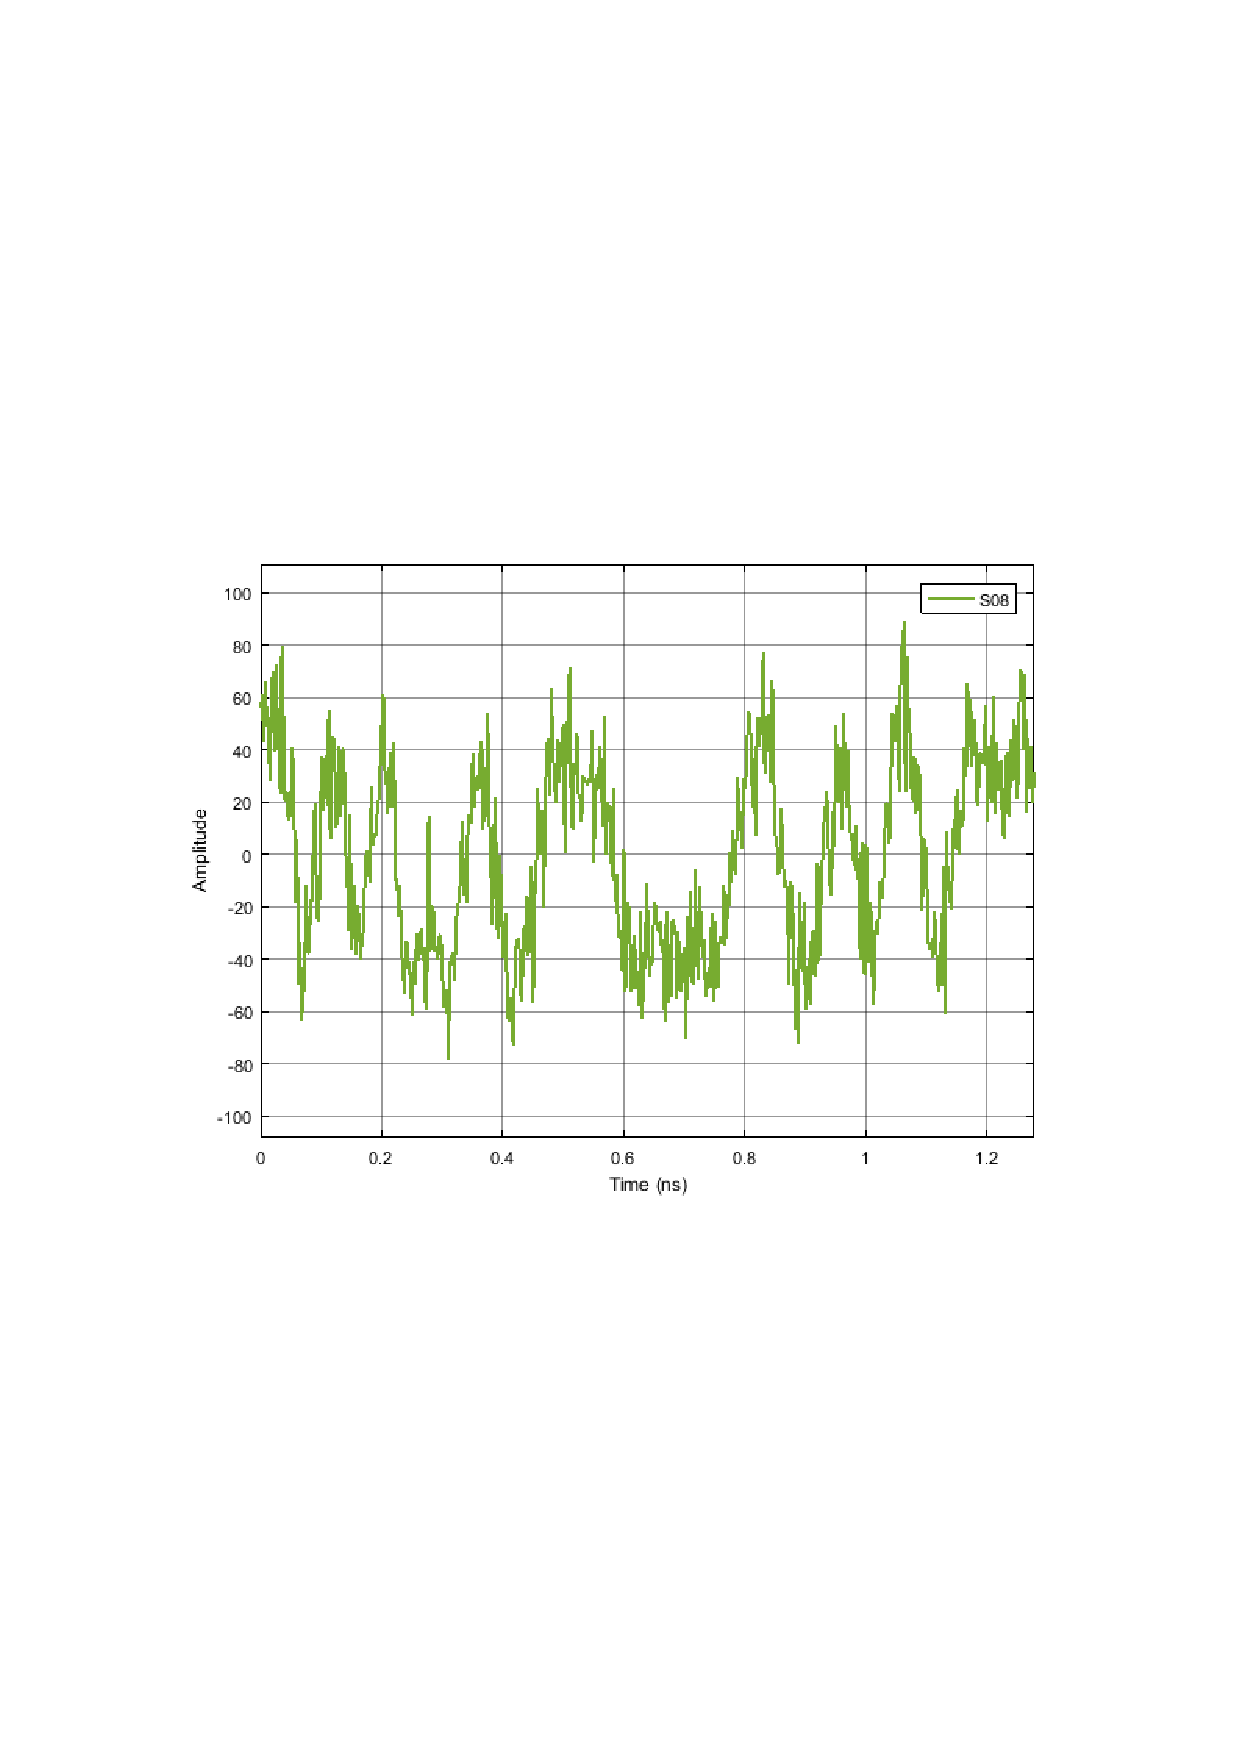
\includegraphics[width=\linewidth, trim= 0mm 95mm 0mm 95mm, clip]{noisy.pdf}
%\caption{Homodyne receiver internal signal: amplification of the signal in Figure~\ref{fig:subtract} with added noise.}
%\label{fig:noisy}
%\end{figure}

%The result of the homodyne detection is the binary string presented in~\ref{fig:decoded}, which is then compared to the original binary string by the BER block, which outputs the report presented in Figure~\ref{fig:ber}.
%
%\begin{figure}[H]
%\centering
%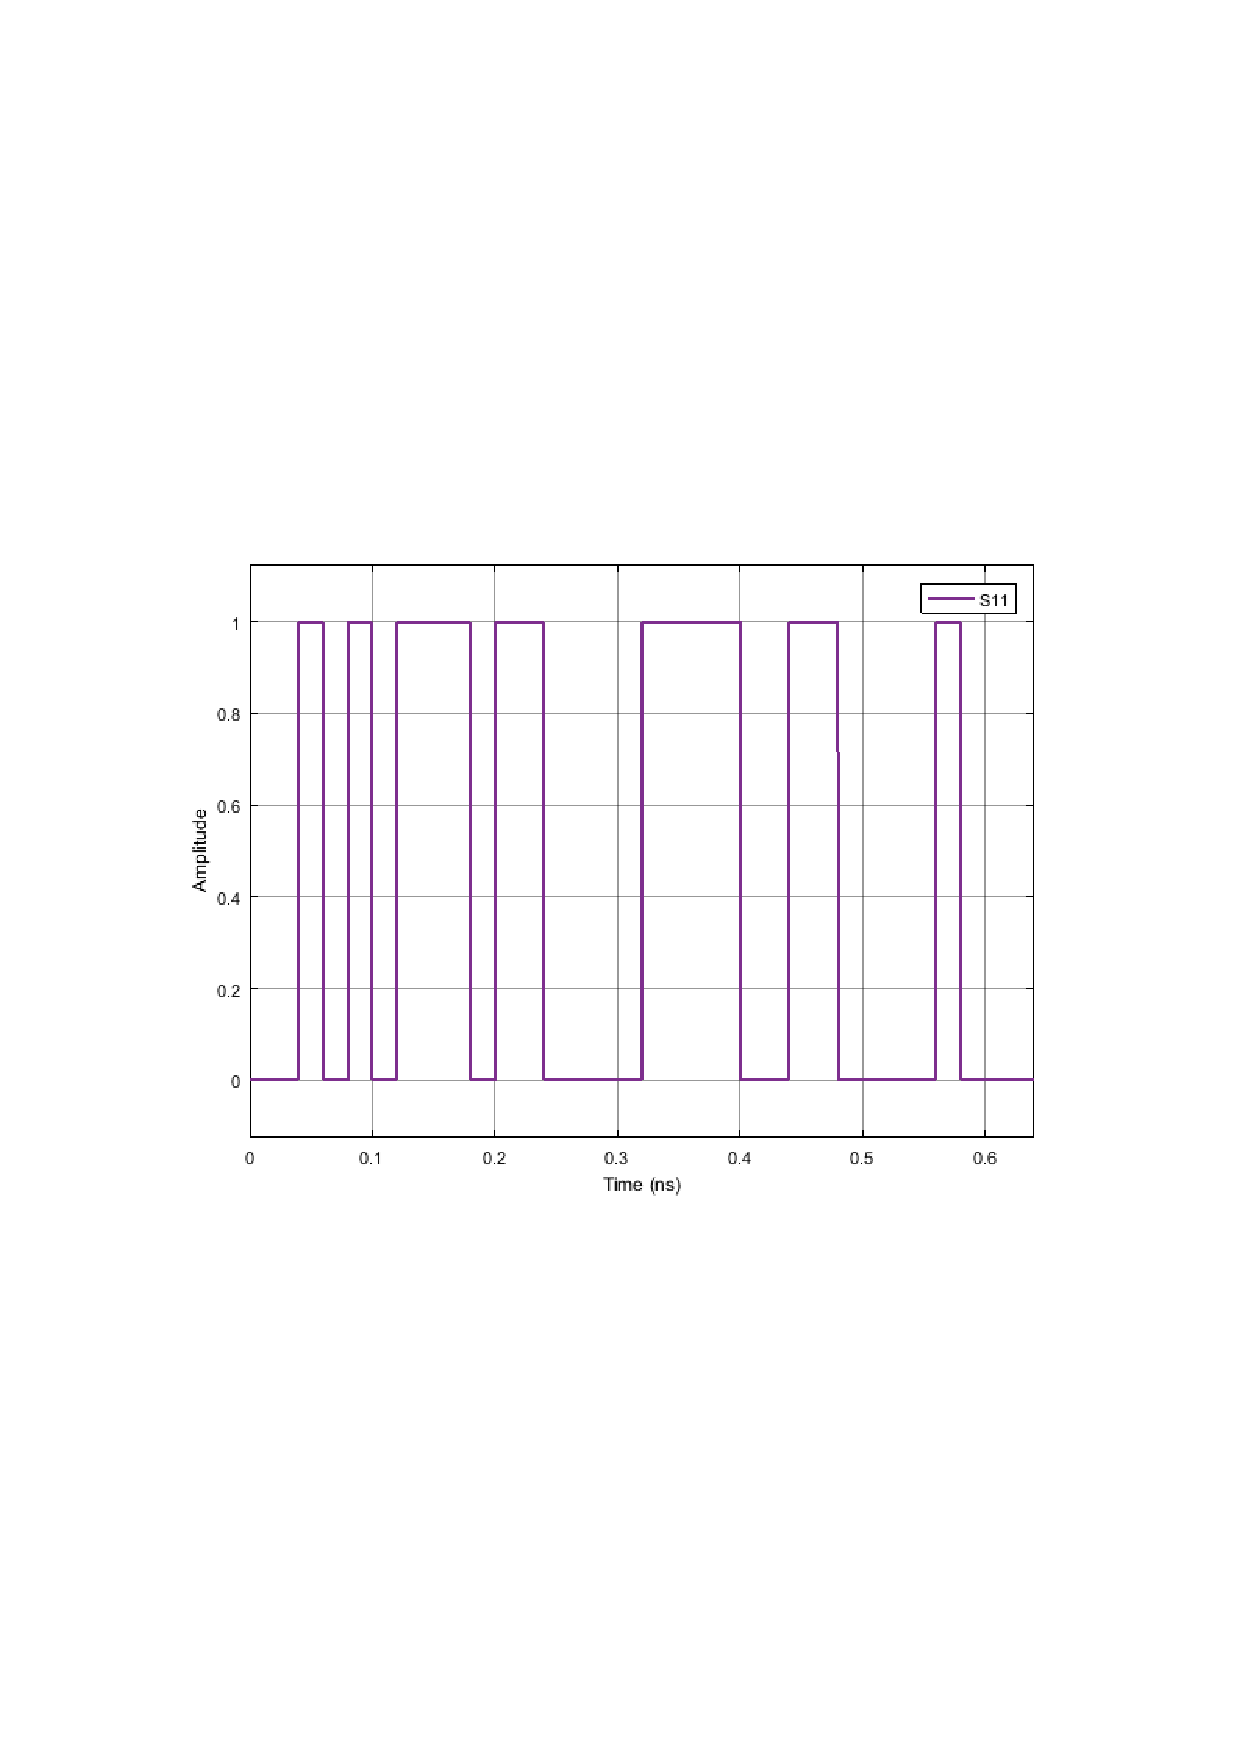
\includegraphics[width=\linewidth, trim= 0mm 95mm 0mm 95mm, clip]{decodedbinarystring.pdf}
%\caption{Decoded binary string, output of the Homodyne receiver block.}
%\label{fig:decoded}
%\end{figure}

%\begin{figure}[H]
%\centering
%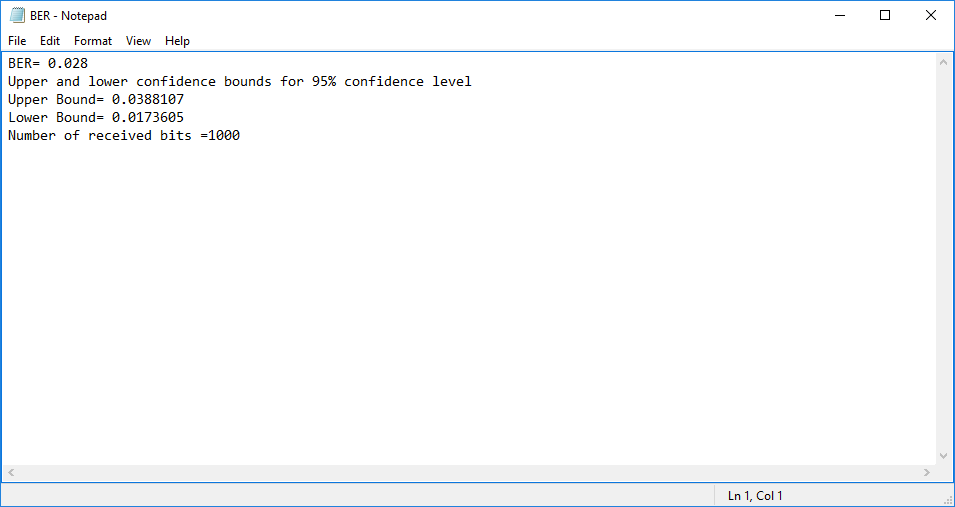
\includegraphics[width=\linewidth]{berreport.png}
%\caption{Bit-Error-Rate report.}
%\label{fig:ber}
%\end{figure}



%\section{Block Description}

%\subsection{MQAM Transmitter}
%% subfile goes here
%
%\subsection{Homodyne Receiver}
%\subfile{../../lib/tex/i_homodyne_reciever}
%
%
%\subsection{Bit Error Rate}
%\subfile{../../lib/tex/ber}
%
%\subsection{Local Oscillator}
%\subfile{../../lib/tex/localoscillator}
%
%\subsection{Beam Splitter}
%\subfile{../../lib/tex/beamsplitter}
%
%\subsection{Photodiode}
%\subfile{../../lib/tex/photodiode}
%
%\subsection{Amplifier}
%\subfile{../../lib/tex/ideal_amplifier}
%
%\subsection{Electrical Filter}
%\subfile{../../lib/tex/pulse_shaper}
%
%\subsection{Sampler}
%\subfile{../../lib/tex/sampler}
%
%\subsection{Bit Decider}
%\subfile{../../lib/tex/decider}
%
%\subsection{Bit Error Rate}
%\subfile{../../lib/tex/ber}

%\section{Known Problems}
%\begin{enumerate}
%    \item{Finish section~\ref{Required files} of this document.}
%    \item{Change figure 1 to increase the lines width and to include the block Sink, and to include the signals names S0, S1, S2, S3.}
%    \item Homodyne Super-Block not functioning
%    \item MQAM Transmitter PDF needs to be written
%    \item 8 bits being lost of every signal
%    \item If the bit string length is larger than 512, this first 512 bits are lost
%\end{enumerate}

%\end{document} 
